%%%%%%%%%%%%%%%%%%%%%%%%%%%%%%%%%%%%%%%%%
% Beamer Presentation
% LaTeX Template
% Version 1.0 (10/11/12)
%
% This template has been downloaded from:
% http://www.LaTeXTemplates.com
%
% License:
% CC BY-NC-SA 3.0 (http://creativecommons.org/licenses/by-nc-sa/3.0/)
%
%%%%%%%%%%%%%%%%%%%%%%%%%%%%%%%%%%%%%%%%%

%----------------------------------------------------------------------------------------
%	PACKAGES AND THEMES
%----------------------------------------------------------------------------------------

\documentclass[9pt]{beamer}
\usepackage{ctex}
\usepackage{xcolor}

\usepackage[utf8]{inputenc}
\usepackage{graphicx}
\usepackage{cmbright}
\usepackage{amsmath}
\usepackage{verbatim}

\usepackage{threeparttable}
\usepackage{tikz}
%\usefonttheme{professionalfonts}
%\setbeamertemplate{itemize/enumerate body begin}{\small} % 设置条目列表中的字体大小为 \small

\usefonttheme{serif}
% The Beamer class comes with a number of default slide themes
% which change the colors and layouts of slides. Below this is a list
% of all the themes, uncomment each in turn to see what they look like.

%\usetheme{default}
%\usetheme{AnnArbor}
\usetheme{Antibes}
%\usetheme{Bergen}
%\usetheme{Berkeley}			% 不错
%\usetheme{Berlin}
%\usetheme{Boadilla}				%跟Szeged很像
%\usetheme{CambridgeUS}  % 不错
%\usetheme{Copenhagen}
%\usetheme{Darmstadt}
%\usetheme{Dresden}         %跟Szeged很像
%\usetheme{Frankfurt}
%\usetheme{Goettingen}
%\usetheme{Hannover}      % 不错
%\usetheme{Ilmenau}
%\usetheme{JuanLesPins}
%\usetheme{Luebeck}
%\usetheme{Madrid}
%\usetheme{Malmoe}         %跟Szeged很像
%\usetheme{Marburg}
% \usetheme{Montpellier}   %跟Szeged很像
%\usetheme[width=2.5cm]{PaloAlto}
%\usetheme{Pittsburgh}
% \usetheme{Rochester}
%\usetheme{Singapore}
% \usetheme{Szeged}  % 点赞
% \usetheme{Warsaw}  % 点赞
% \setbeamertemplate{title page}[default][colsep=-4bp,rounded=false]


% As well as themes, the Beamer class has a number of color themes
% for any slide theme. Uncomment each of these in turn to see how it
% changes the colors of your current slide theme.
%\definecolor{mycolor}{rgb}{.8,.0,.3}
%\setbeamercolor*{palette primary}{use=structure,fg=white,bg=mycolor}
%\usecolortheme{albatross}
%\usecolortheme{beaver}
%\usecolortheme{beetle}
%\usecolortheme{crane}
%\usecolortheme{dolphin}
%\usecolortheme{dove}
%\usecolortheme{fly}
%\usecolortheme{lily}
%\usecolortheme{orchid}
% \usecolortheme{rose}
%\usecolortheme{seagull}
%\usecolortheme{seahorse}
%\usecolortheme{whale}
%\usecolortheme{wolverine}
%\usecolortheme[named=mycolor]{structure}
%\setbeamertemplate{footline} % To remove the footer line in all slides uncomment this line
%\setbeamertemplate{footline}[page number] % To replace the footer line in all slides with a simple slide count uncomment this line

%\setbeamertemplate{navigation symbols}{} % To remove the navigation symbols from the bottom of all slides uncomment this line


\usepackage{booktabs} % Allows the use of \toprule, \midrule and \bottomrule in tables

%----------------------------------------------------------------------------------------
%	TITLE PAGE
%----------------------------------------------------------------------------------------

\title{\songti 从强化学习到择时策略} % The short title appears at the bottom of every slide, the full title is only on the title page

\author{朱大福} % Your name
\institute[School of Economics (SOE)\\
Wang Yanan Institute for Studies in Economic \\ Xiamen University] % Your institution as it will appear on the bottom of every slide, may be shorthand to save space

\date{2024/07/09} % Date, can be changed to a custom date

\begin{document}
\songti
\begin{frame}
\titlepage % Print the title page as the first slide
\end{frame}
%
%\begin{frame}
%\frametitle{Overview} % Table of contents slide, comment this block out to remove it
%\tableofcontents[hideallsubsections] % Throughout your presentation, if you choose to use \section{} and \subsection{} commands, these will automatically be printed on this slide as an overview of your presentation
%\end{frame}

%----------------------------------------------------------------------------------------
%	PRESENTATION SLIDES
%----------------------------------------------------------------------------------------

%------------------------------------------------
% Sections can be created in order to organize your presentation into discrete blocks, all sections and subsections are automatically printed in the table of contents as an overview of the talk
%------------------------------------------------

 % A subsection can be created just before a set of slides with a common theme to further break down your presentation into chunks


%------------------------------------------------
%------------------------------------------------

\section{WISERCLUB分享内容}
\begin{frame}
\begin{figure}
\centering
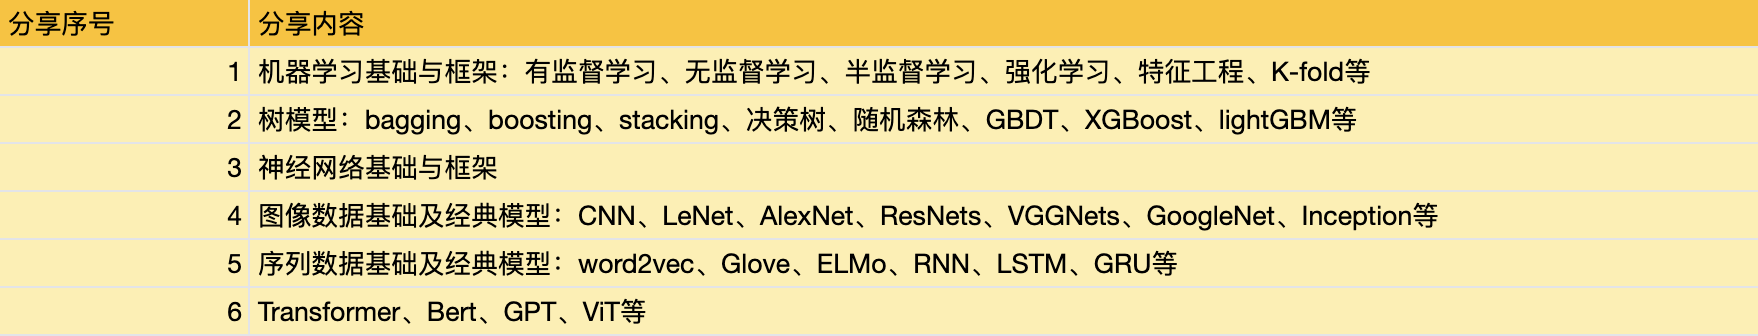
\includegraphics[width=10cm]{../fig/上学期.png}
\label{}

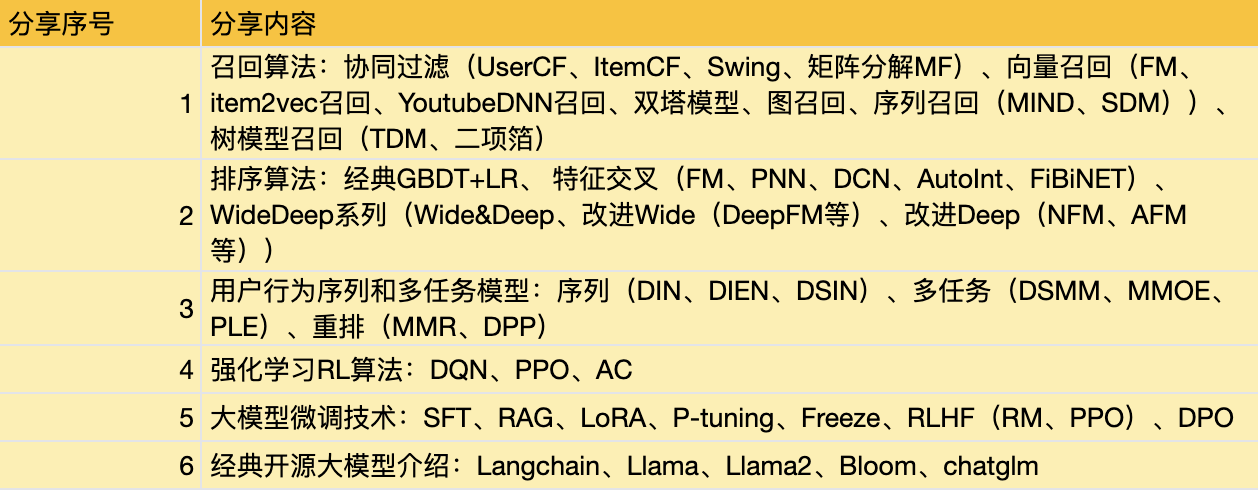
\includegraphics[width=10cm]{../fig/下学期.png}
\caption{机器学习小组}

\end{figure}
\end{frame}

\begin{frame}
\begin{figure}
\centering
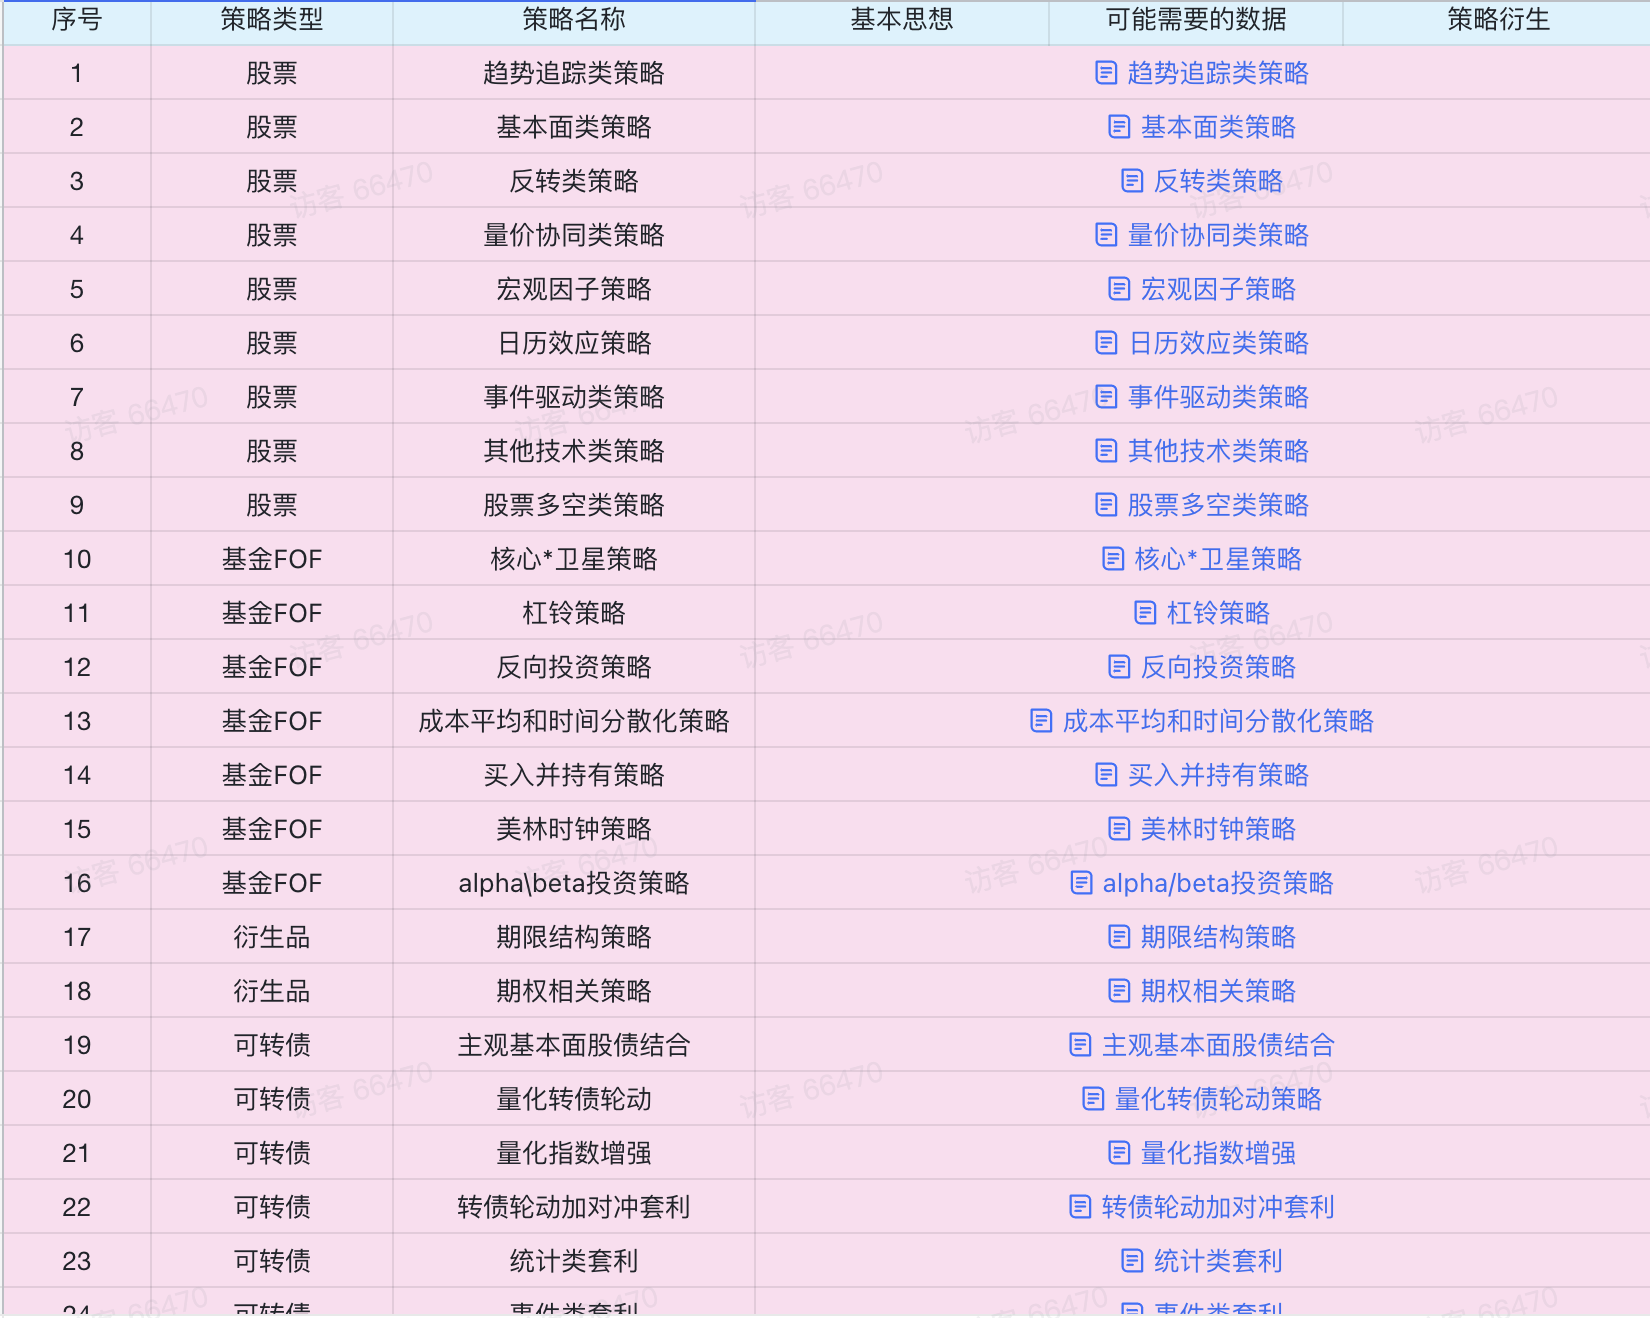
\includegraphics[width=9cm]{../fig/量金.png}
\caption{量化金融小组}

\end{figure}
\end{frame}



\section{机器学习的分类}
\begin{frame}

机器学习:Data-driven

\vspace{1em}

\frametitle{几类学习问题}
\begin{itemize}
\item 有监督学习
\begin{itemize}
\item Data: $(x,y)$
\item 目标:$x\rightarrow y$
\begin{figure}

\includegraphics[height=3em]{../fig/apple1.png}

\end{figure}
\end{itemize}\pause

\item 无监督学习
\begin{itemize}
\item Data: $x$
\item 目标:$x_1$和$x_2$是同类
\begin{figure}
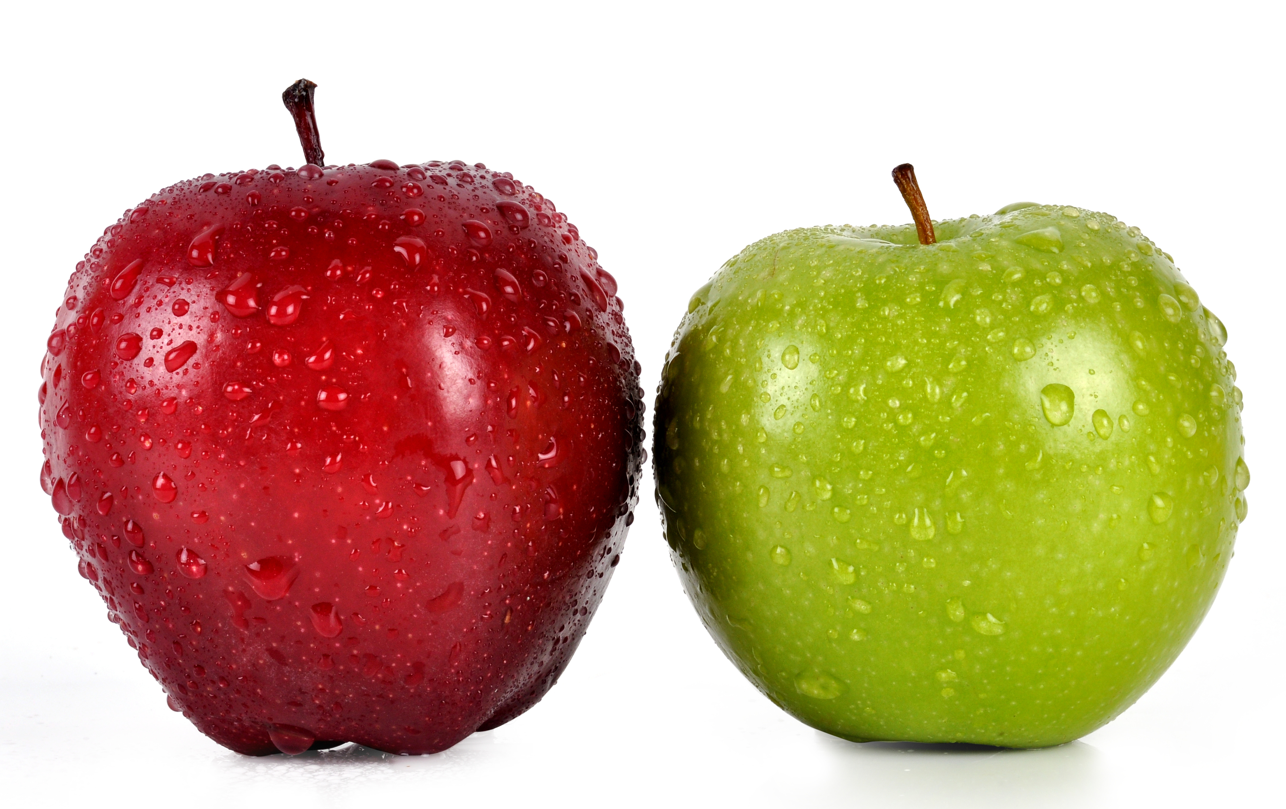
\includegraphics[height=3em]{../fig/apple2.png}\pause

\end{figure}
\end{itemize}

\item 强化学习
\begin{itemize}
\item Data: $(s,a)$
\item 目标:回报最大化
\begin{figure}

\includegraphics[height=6em]{../fig/apple3.png}

\end{figure}
\end{itemize}

\end{itemize}

\end{frame}

%------------------------------------------

\section{强化学习基本概念}
\begin{frame}
\frametitle{交互环境}

\begin{figure}
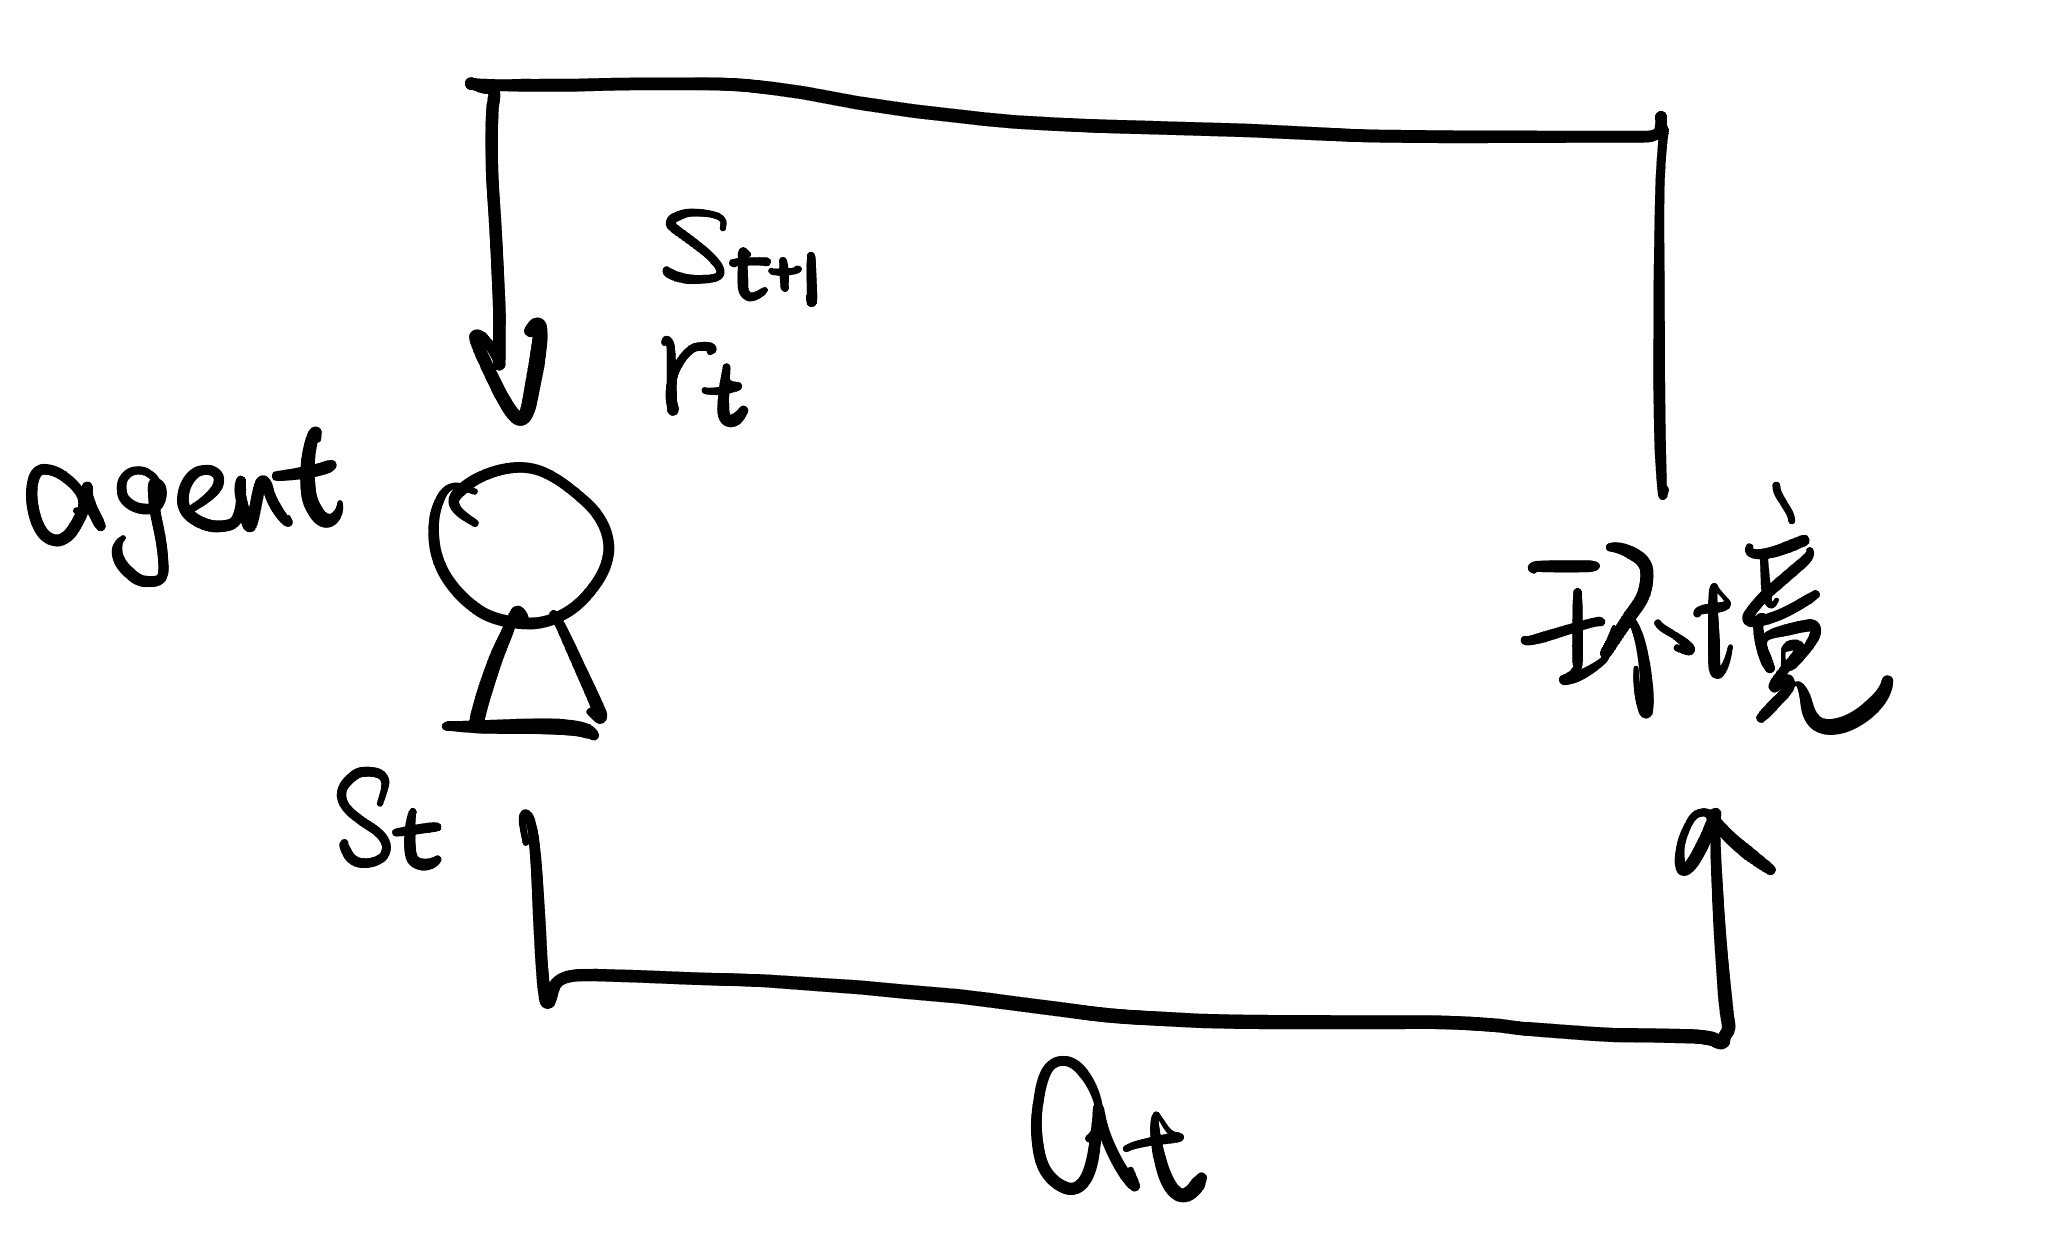
\includegraphics[width=6cm]{../fig/agent.jpg}
\caption{agent与环境交互}
\end{figure}

回报:$R_t=r_t+\gamma\cdot r_{t+1}+\gamma^2\cdot r_{t+2}+\cdots$

\end{frame}


\begin{frame}
\frametitle{定义价值函数}

Notation

\begin{itemize}
\item $s$为现在的状态
\item $s'$为下一期的状态
\item $a$为现在的动作
\item $a'$为下一期的动作
\end{itemize}

\vspace{1em}

\[
V(s)=\mathbb{E}[R_t|s]
\]

\[
Q(s,a)=\mathbb{E}[R_t|s,a]
\]

By Law of Total Probability

\[
V(s)=\mathbb{E}\bigg[\mathbb{E}[R_t|s,a]\bigg]=\mathbb{E}[Q(s,a)]
\]

\end{frame}

\begin{frame}
\frametitle{策略学习与价值学习}

策略:$a\sim \pi(\cdot|s)$

\vspace{1em}

\begin{enumerate}

\item 策略学习(policy learning)
\begin{itemize}
\item 找 $\pi(\cdot|s)$
\item 特点:动作a连续
\end{itemize}

\pause

\vspace{1em}

\item 价值学习(value learning)
\begin{itemize}
\item 找 $Q(s,a)$
\item 策略是选择让Q值最大的动作
\[
a=\arg\max_a Q(s,a)
\]

\end{itemize}

\end{enumerate}

\end{frame}

\begin{frame}
\frametitle{价值学习}

\begin{figure}
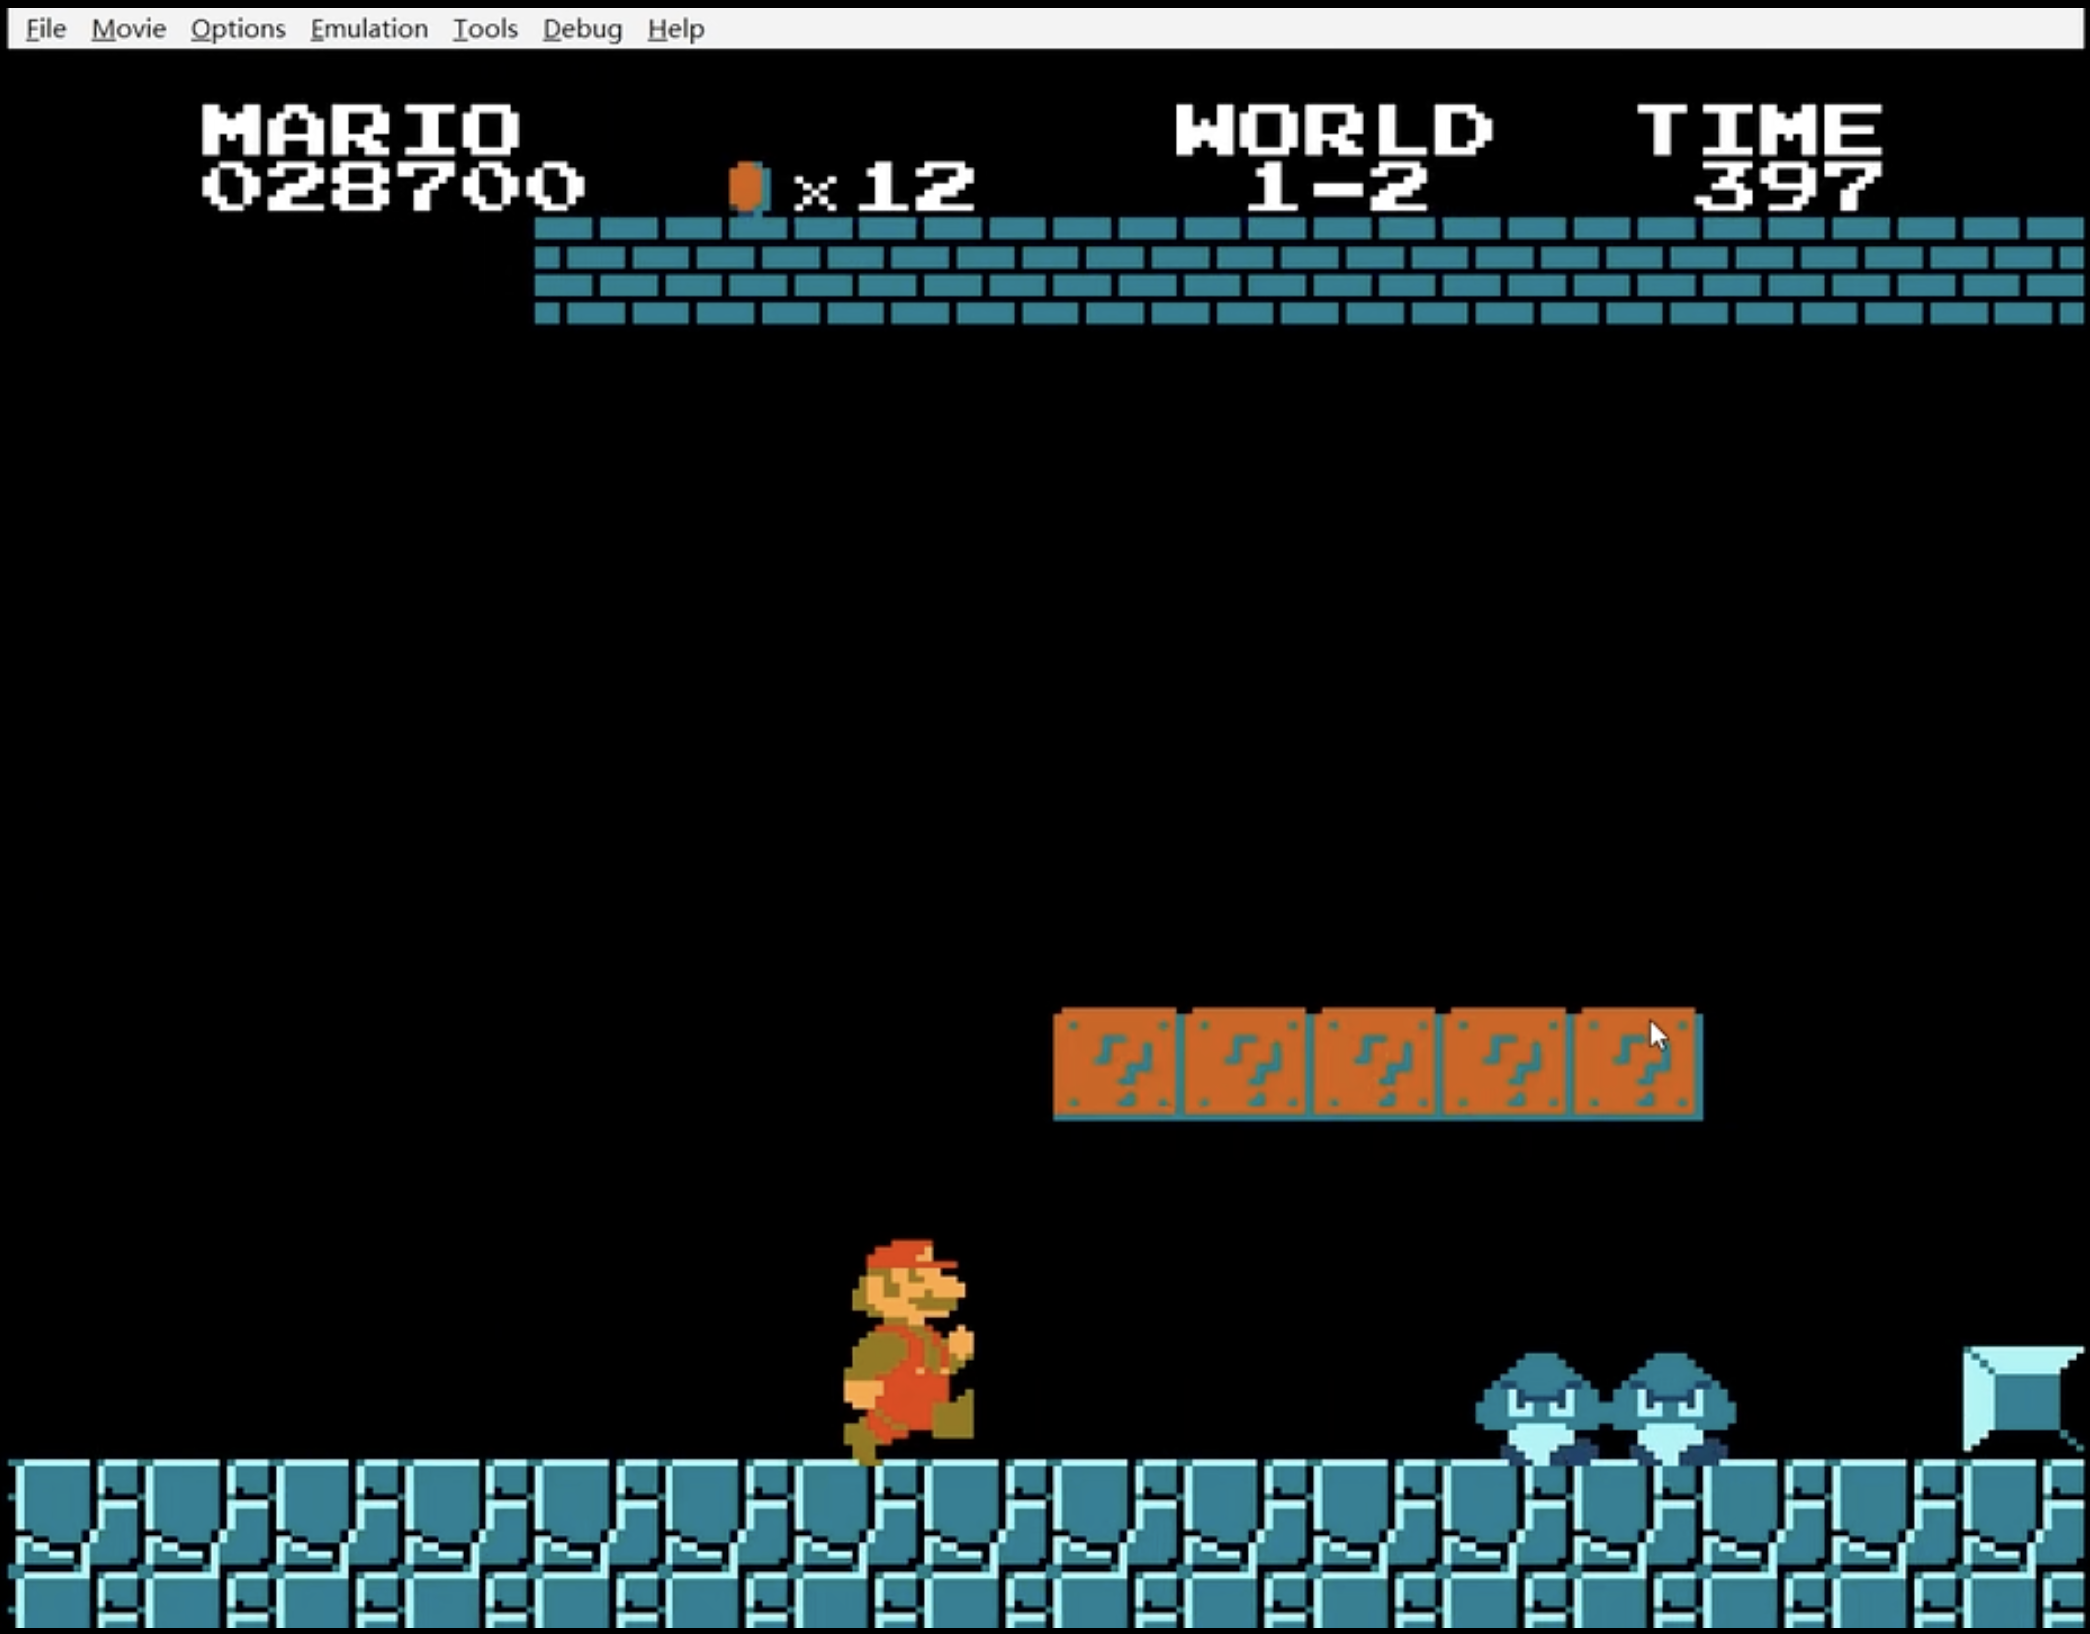
\includegraphics[width=6cm]{../fig/mario.png}
\end{figure}

\[
a=\{\text{右}, \text{上}, \text{左}\}
\]

\end{frame}

\begin{frame}
\frametitle{价值学习}

\begin{figure}
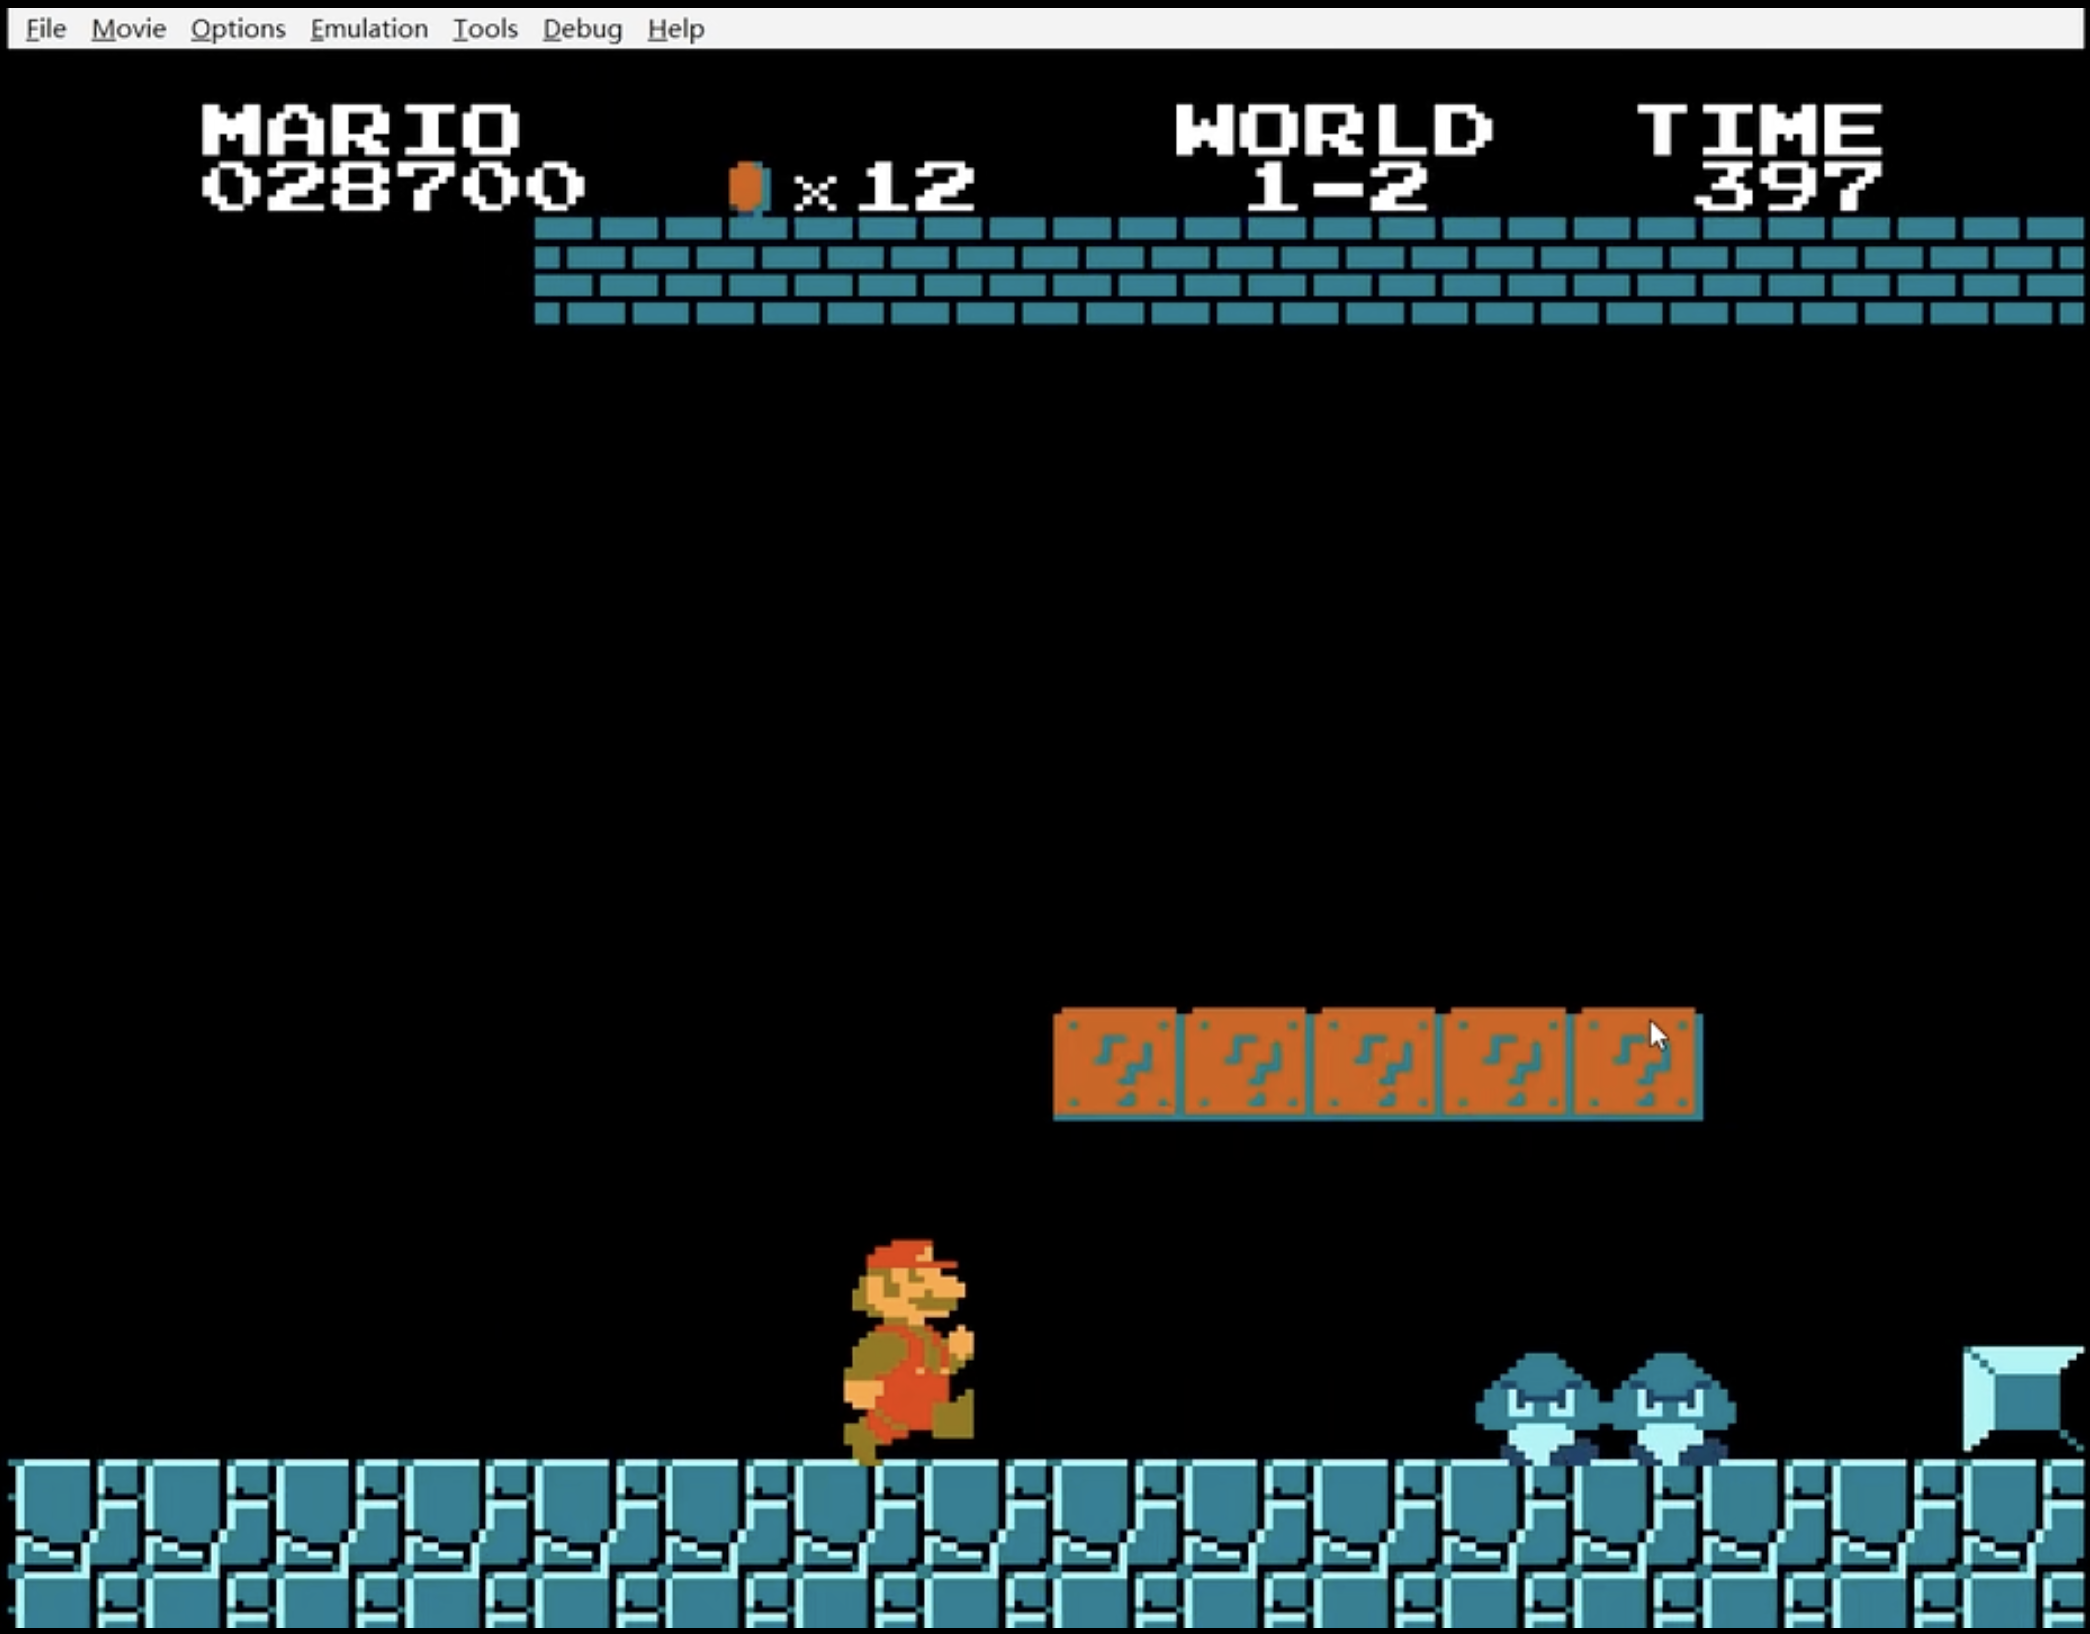
\includegraphics[width=6cm]{../fig/mario.png}
\end{figure}

\[
Q(s,\text{右})=100,\quad Q(s,\text{上})=50, \quad Q(s,\text{左})=-30
\]

% 适合表格数据

\end{frame}

\begin{frame}
\frametitle{Agent交互的随机性}

\begin{figure}
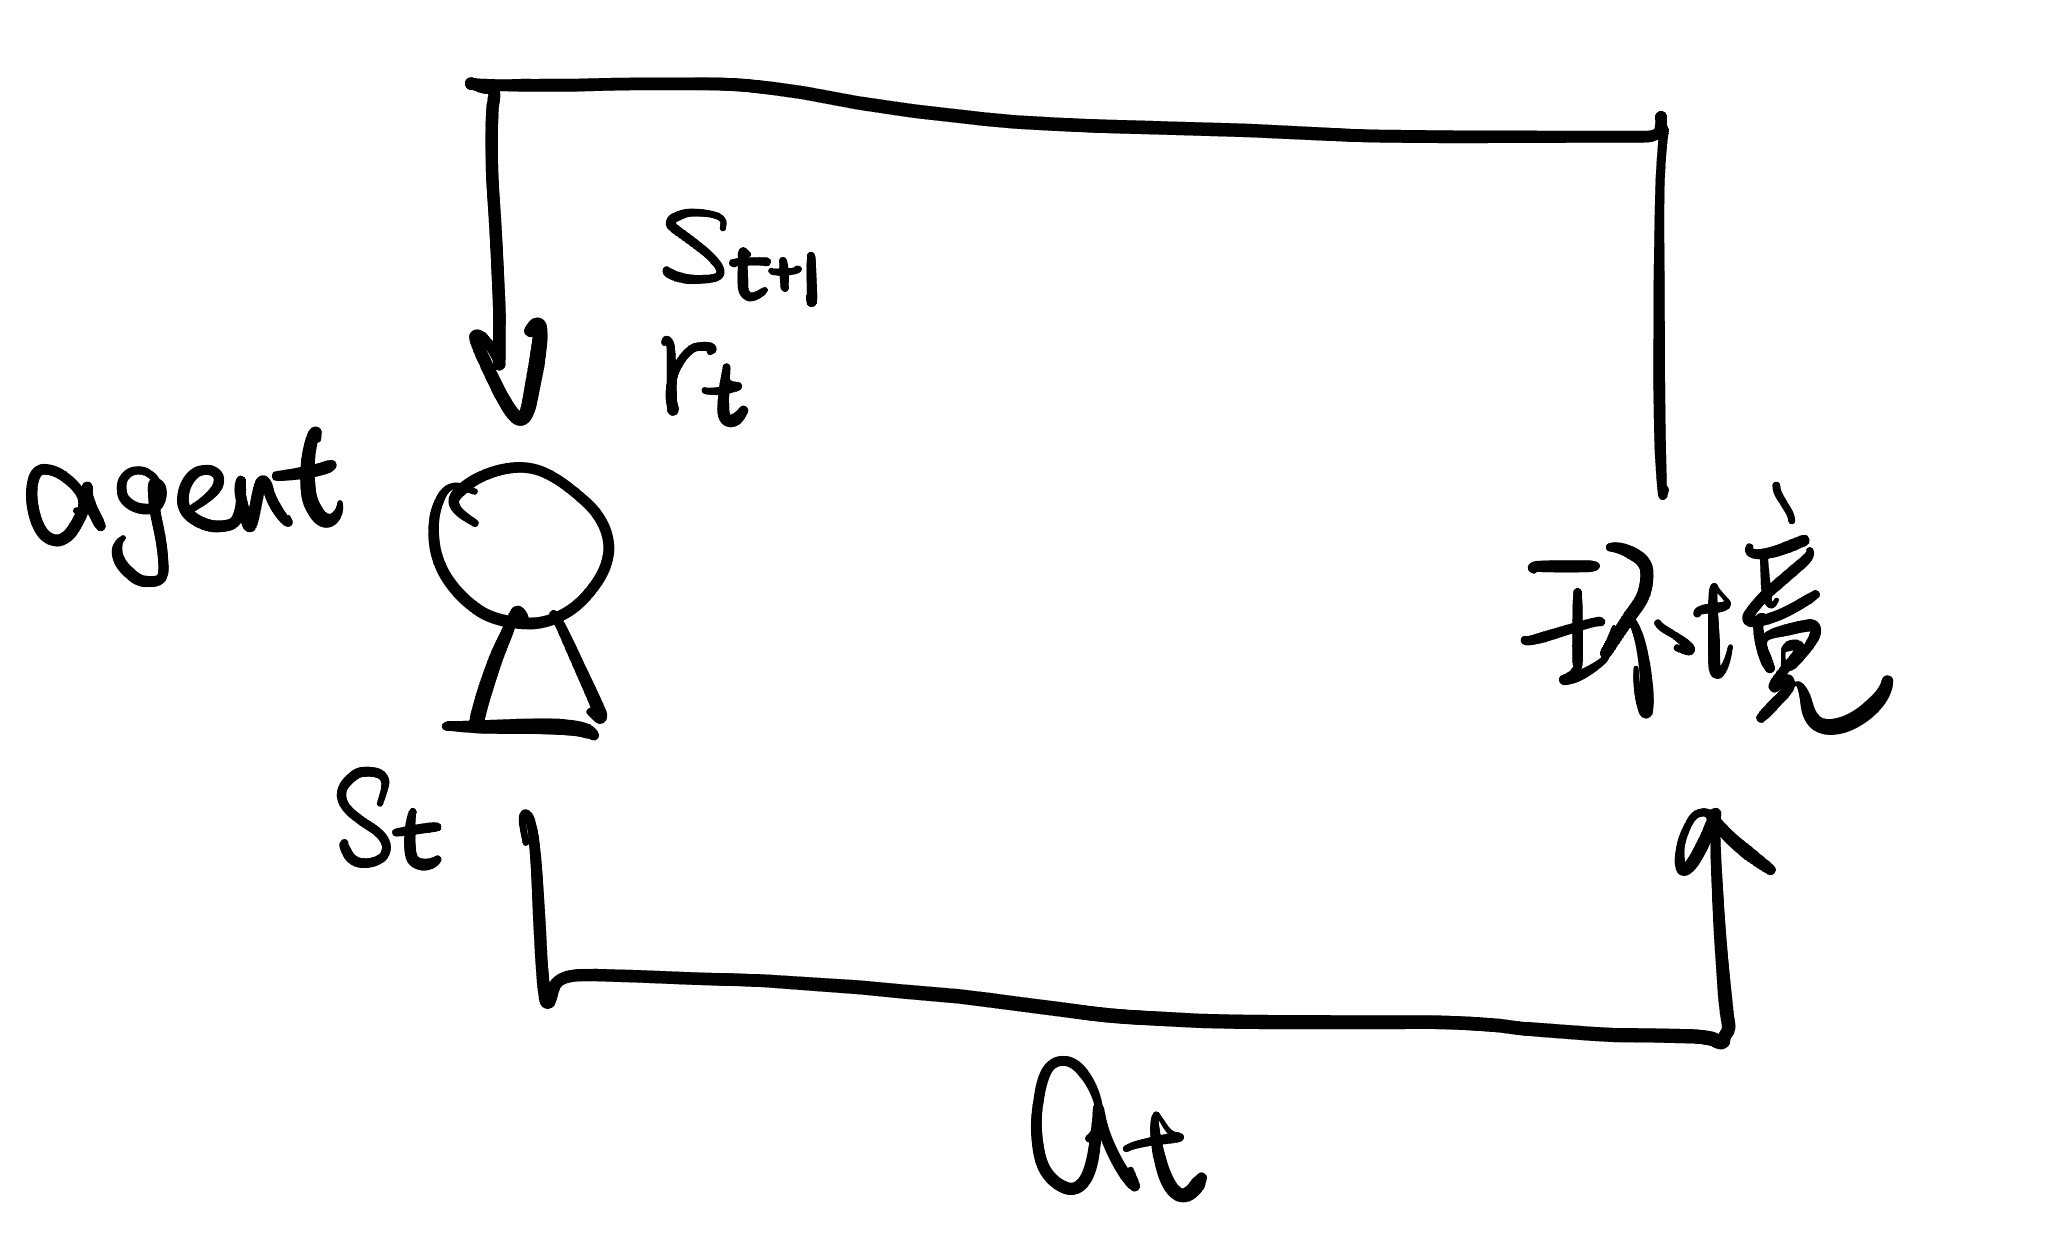
\includegraphics[width=4cm]{../fig/agent.jpg}
\end{figure}

\begin{enumerate}
\item 此时状态为$s$,做什么动作$a$? $\Rightarrow$ 由Agent决定

\[
\pi(a|s)
\]

\item 此时状态为$s$并做出动作$a$,下一刻是什么状态$s'$? $\Rightarrow$ 由环境决定

\[
P(s'|s,a)
\]
\end{enumerate}

\end{frame}

\begin{frame}
\frametitle{贝尔曼方程}

Bellman equation

\[
Q(s,a)=r(s,a)+\gamma\cdot \sum_{s'\in \mathcal{S}}P(s'|s,a)\underbrace{\left[\sum_{a'\in \mathcal{A}}\pi(a'|s')Q(s',a') \right]}_{V(s')}
\]

Optimal Bellman equation

\vspace{1em}

\[
Q^*(s,a)=r(s,a)+\gamma\cdot \sum_{s'\in \mathcal{S}}P(s'|s,a)\max_{a'}Q(s',a')
\]

\pause

\vspace{1em}

价值学习!策略是选最大的Q的动作

\end{frame}

\begin{frame}
\frametitle{Q-learning}

\[
Q^*(s,a)=r(s,a)+\gamma\cdot \sum_{s'\in \mathcal{S}}P(s'|s,a)\max_{a'}Q(s',a')
\]

\vspace{1em}


$P(s'|s,a)$ 未知,怎么办?\pause

\vspace{1em}


如果$\{a=\text{上}\}$,在$n=1000$次交互中

\[
s'=\begin{cases}
\text{通过} & n=900\\
\text{失败} & n=100
\end{cases}
\quad 
\xrightarrow{\text{近似}} 
\quad 
P(s'|s,a)= \begin{cases}
0.9 & s'=\text{通过}\\
0.1 & s'=\text{失败}
\end{cases}
\]

\end{frame}

\section{DQN与Q-learning}
\begin{frame}
\frametitle{Q-learning}

\[
Q^*(s,a)=r(s,a)+\gamma\cdot \max_{a'}Q(s',a')
\]

初始化$\hat{Q}(\cdot)$

\[
\hat{Q}(s,a)\leftarrow \hat{Q}(s,a)+\alpha \left [ Q^*(s,a)-\hat{Q}(s,a) \right]
\]

\vspace{1em}

\end{frame}

\begin{frame}
\frametitle{Deep Q Network}

当状态的每一个维度都连续时,无法用表格记录

\vspace{1em}

$\rightarrow$ 函数拟合

\begin{figure}
\centering
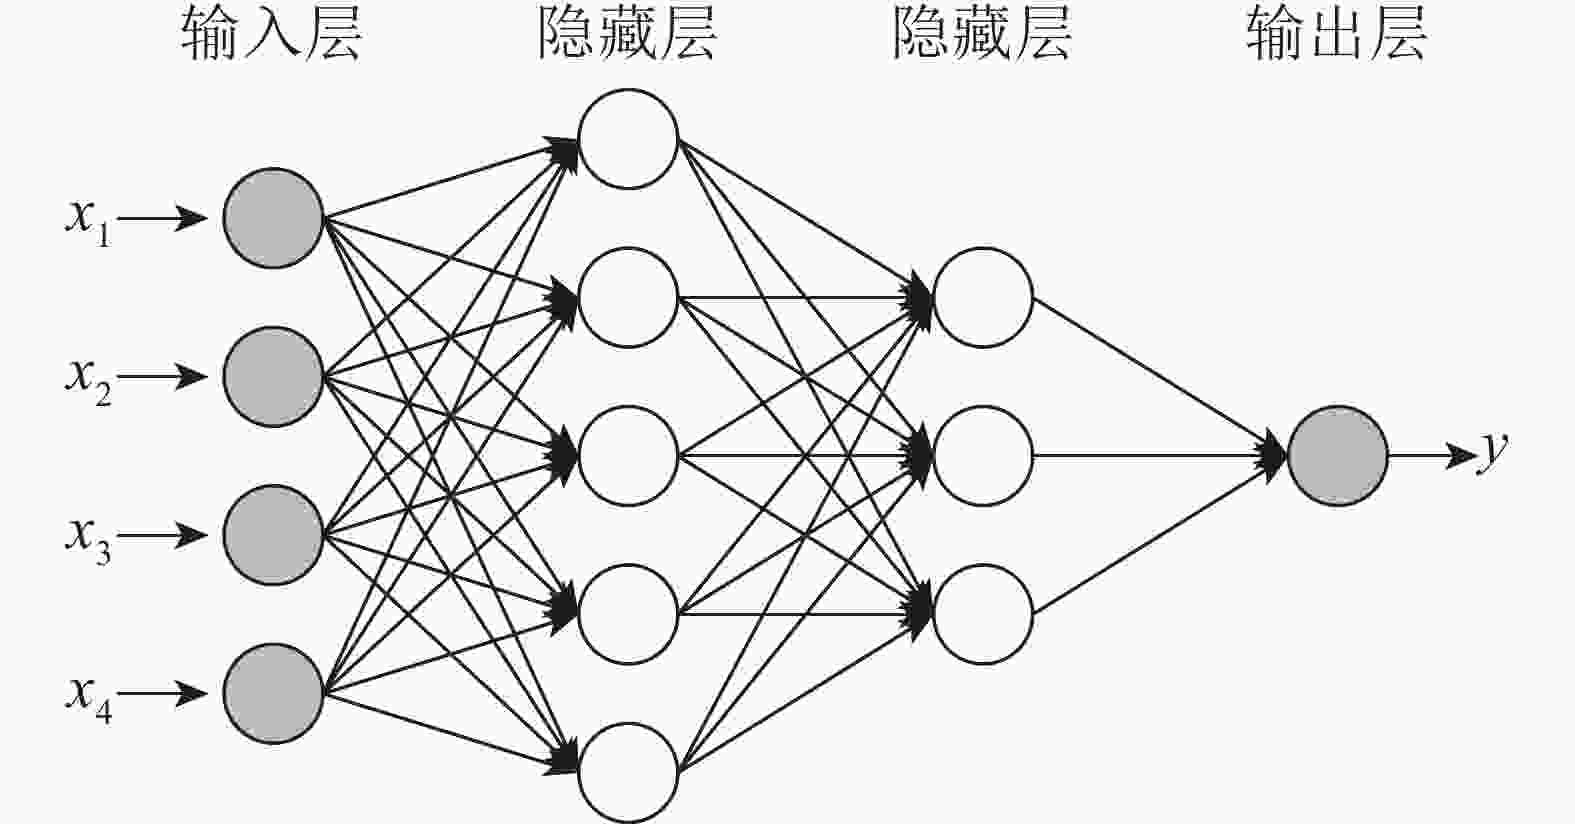
\includegraphics[width=8cm]{../fig/nn.jpg}
\caption{神经网络}
\end{figure}

\end{frame}

%%%% 

\begin{frame}
\frametitle{Deep Q Network}

怎样训练DQN?\pause

\vspace{1em}

\begin{figure}
\centering
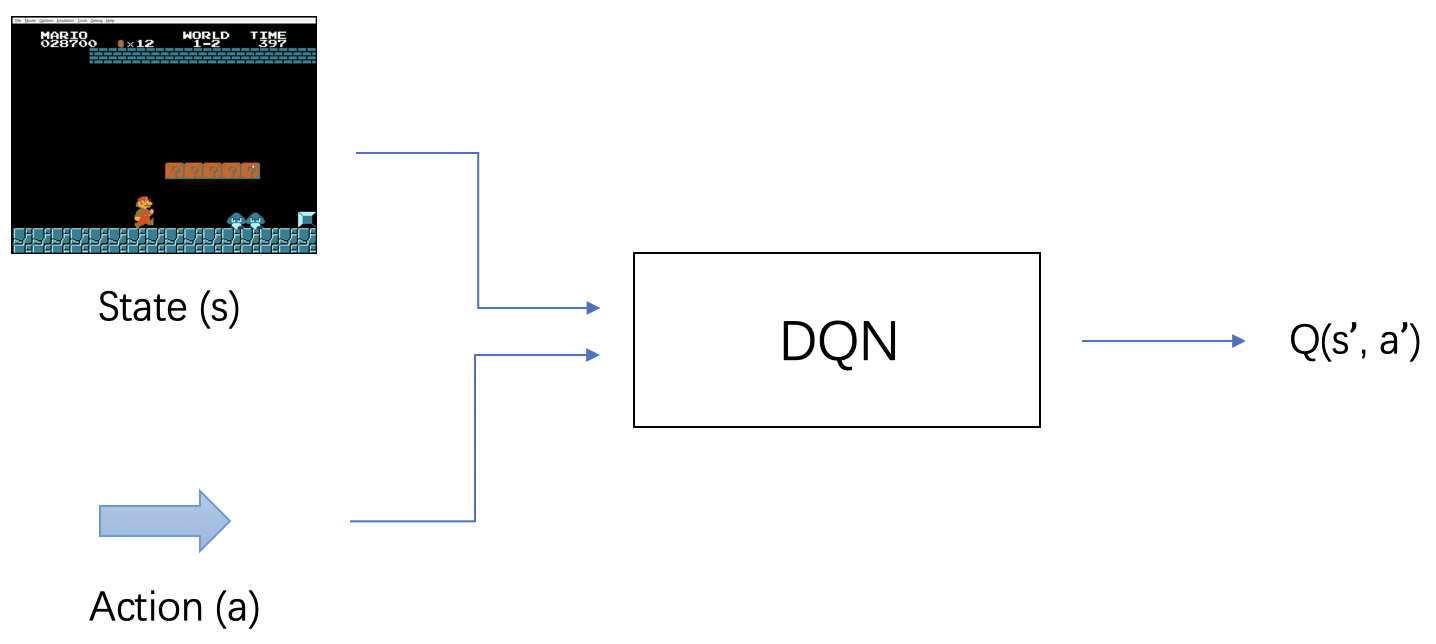
\includegraphics[width=7cm]{../fig/s+a.png}
\pause
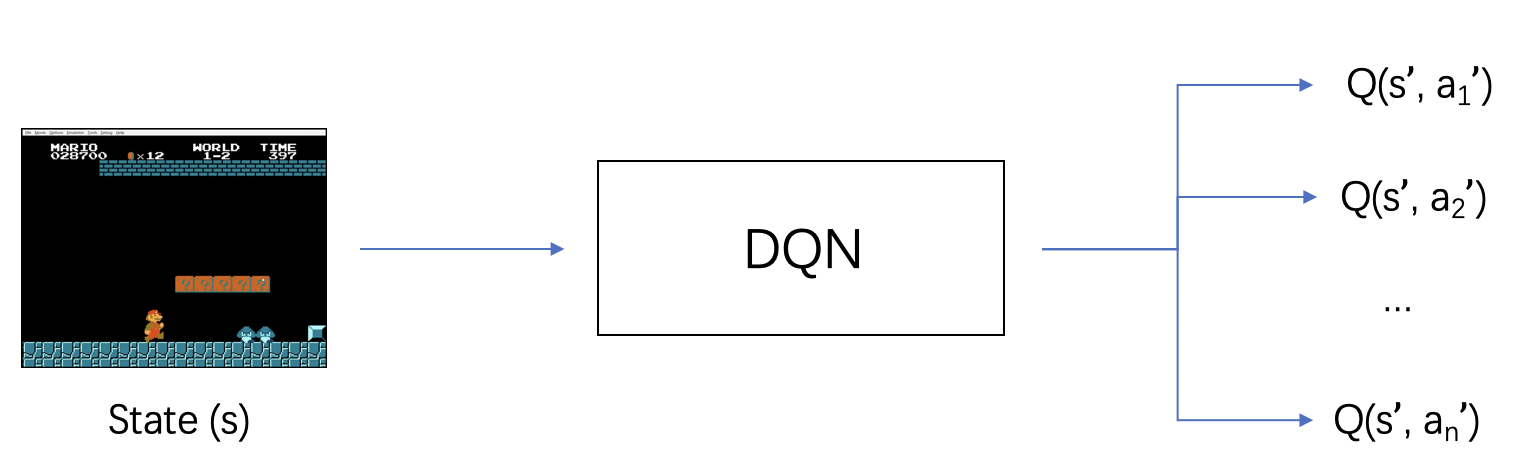
\includegraphics[width=7.5cm]{../fig/s.png}
\end{figure}

\end{frame}

\begin{frame}
\frametitle{Deep Q Network}

训练目标:

\[
r(s,a)+\gamma \cdot \max_{a'} Q(s',a')
\]

预测值:

\[
Q(s,a)
\]

损失函数

\[
\mathcal{L}=\mathbb{E}\left[ \bigg\Vert Q(s,a) - \left( r(s,a)+\gamma \cdot \max_{a'} Q(s',a')\right)\bigg\Vert^2 \right]
\]

\end{frame}

\begin{frame}
\frametitle{Deep Q Network}

\begin{itemize}
\item 经验回放(experience replay)

\[
(s,a,r,s')\rightarrow \text{缓冲回放区}
\]

\item 目标网络

\[
Q(s,a)\leftarrow Q(s,a)+\alpha \left [ \left(r(s,a) + \gamma \max_{a'\in A}Q(s',a')\right)-Q(s,a) \right]
\]

\[
\max_{a'\in A}Q(s',a')\rightarrow \max_{a'\in A}Q_-(s',a')
\]

\end{itemize}

\end{frame}

\section{研报复现}
\begin{frame}
\frametitle{DQN择时策略}

数据:

上证指数 2007-01-04至 2022-06-30日度行情数据。其中 2007至 2016年为训练集,用来训练智能体; 2017 至 2022 年为测试集, 用来评估智能体表现。

状态空间$\mathcal{S}$: 
\begin{itemize}
\item 日度开盘价、最高价、最低价、收盘价
\item 标准化处理
\item 设置回看区间 $lookback=5$,一个状态为$lookback\times 4$的张量
\end{itemize}

\vspace{1em}


动作空间$\mathcal{A}$

\[
\mathcal{A}=\{buy, sell, hold\}
\]

\end{frame}

\begin{frame}
\frametitle{DQN择时策略}

奖励$\mathcal{R}$

\begin{figure}
\centering
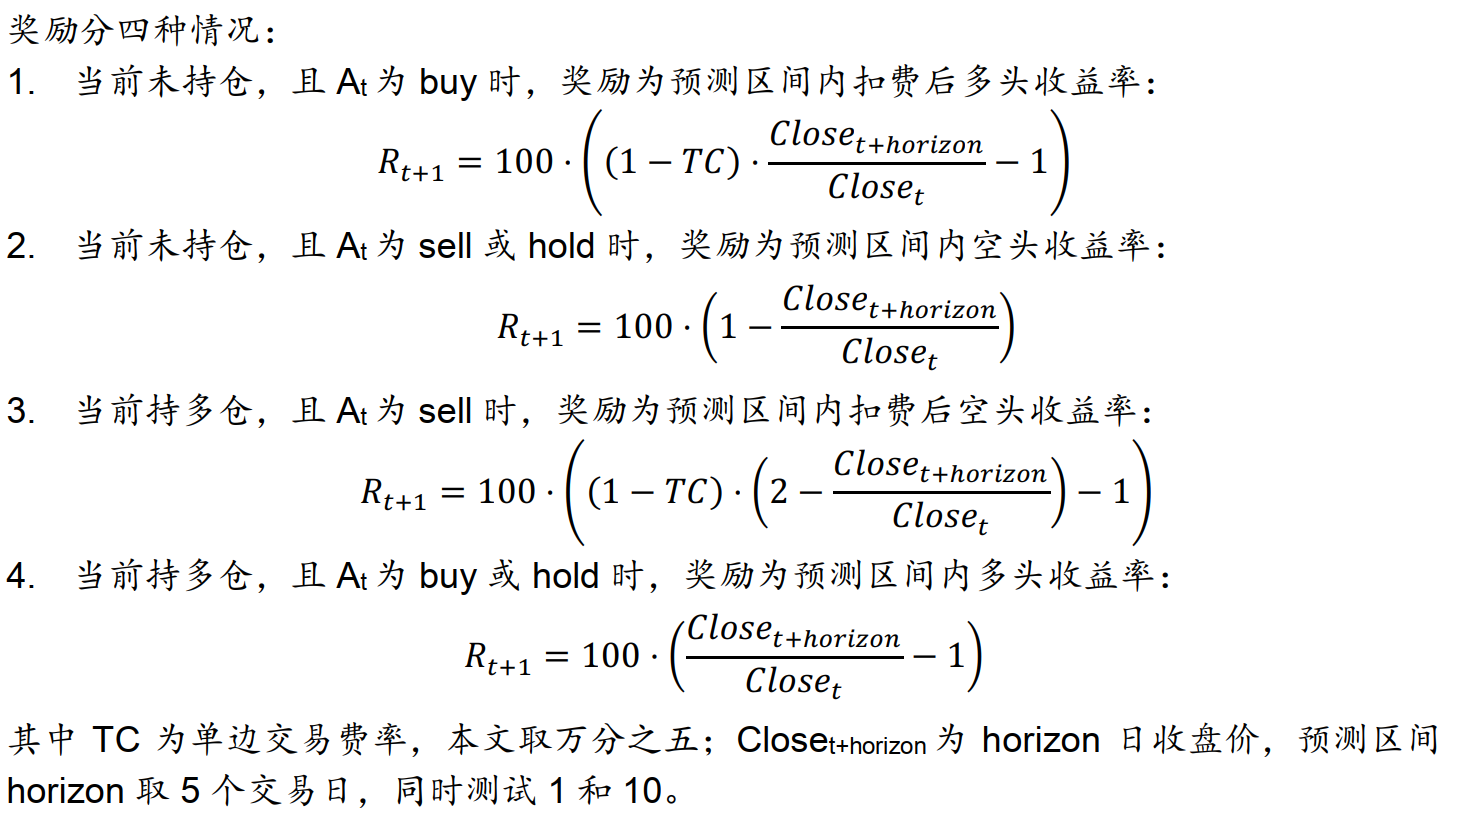
\includegraphics[width=10cm]{../fig/R.png}
\end{figure}

\end{frame}

\begin{frame}
\frametitle{DQN择时策略}
\begin{figure}
\centering
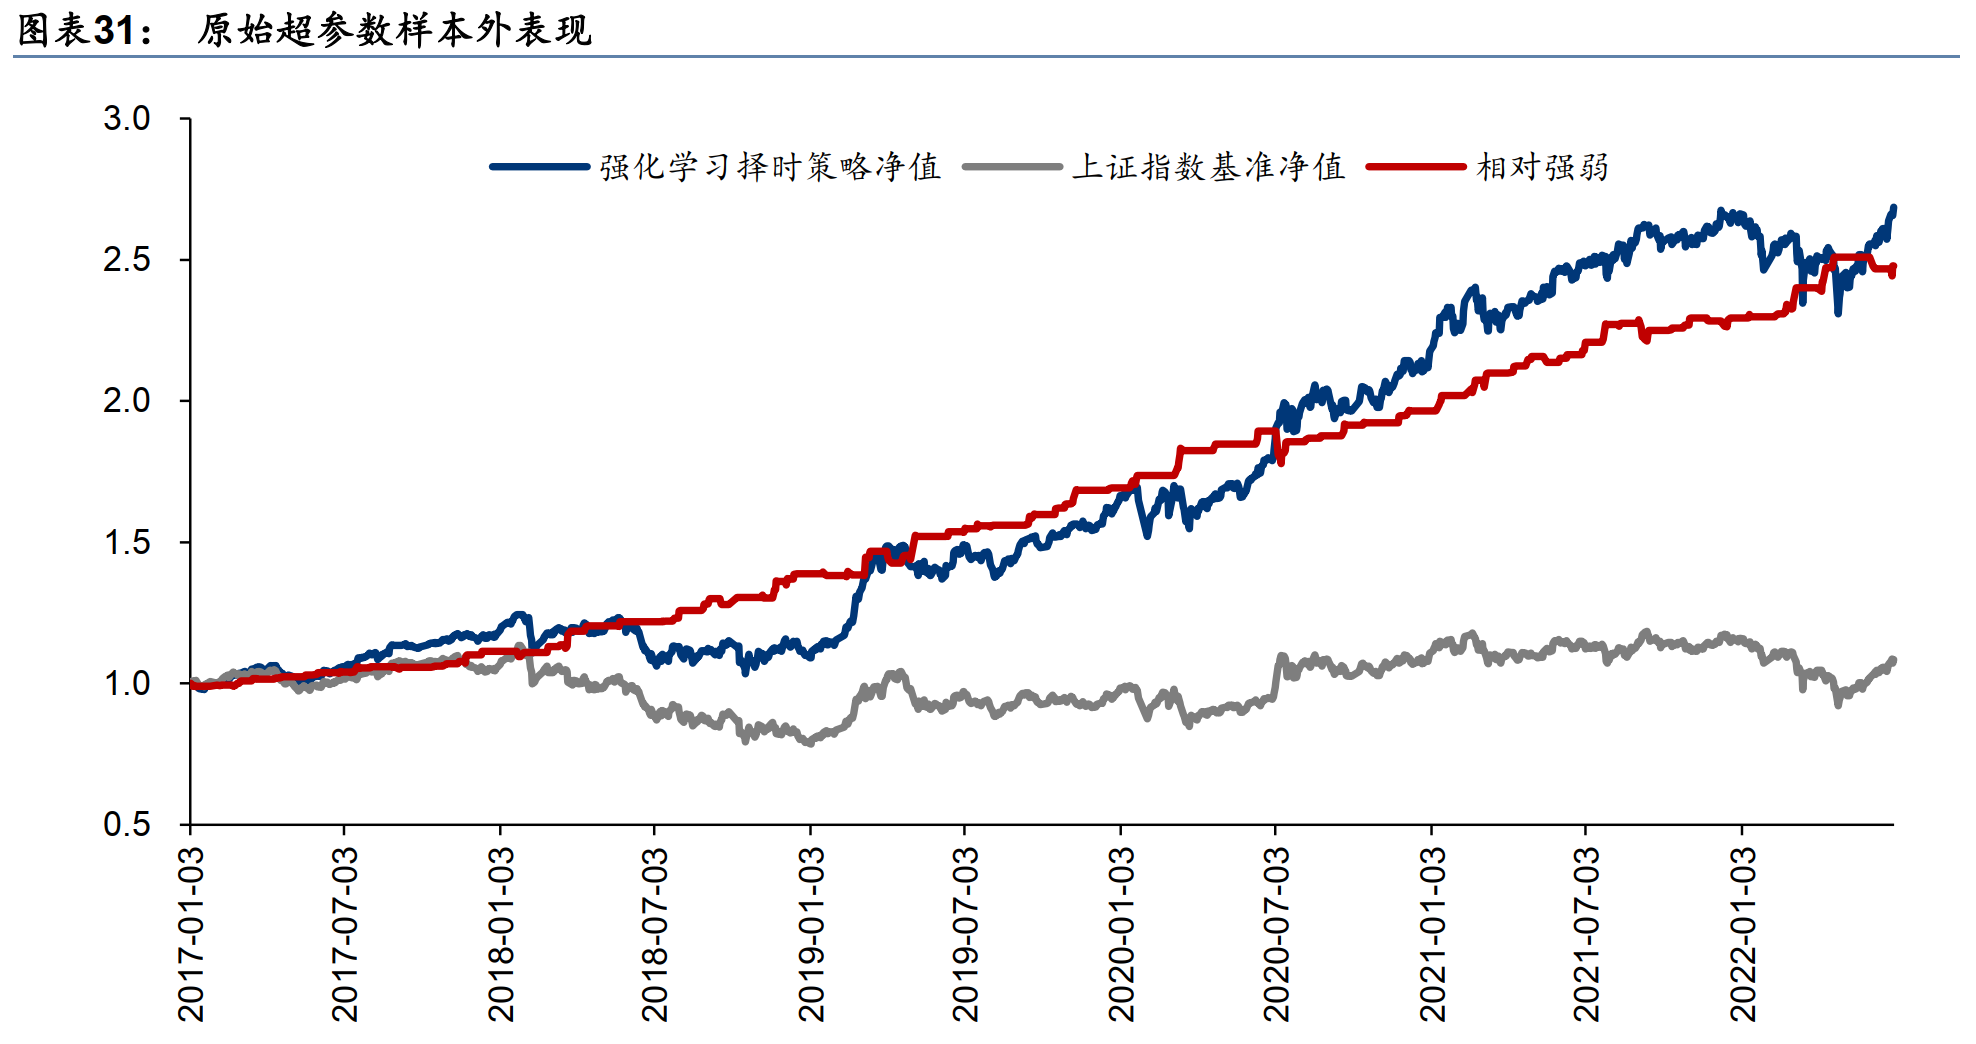
\includegraphics[width=10cm]{../fig/pnl.png}
\end{figure}
\end{frame}

\begin{frame}
\frametitle{一点反思}

\begin{itemize}
\item 特征
\item 更复杂的模型:Actor-Critic, TRPO, PPO, DDPG, SAC...
\end{itemize}

\begin{figure}
\centering
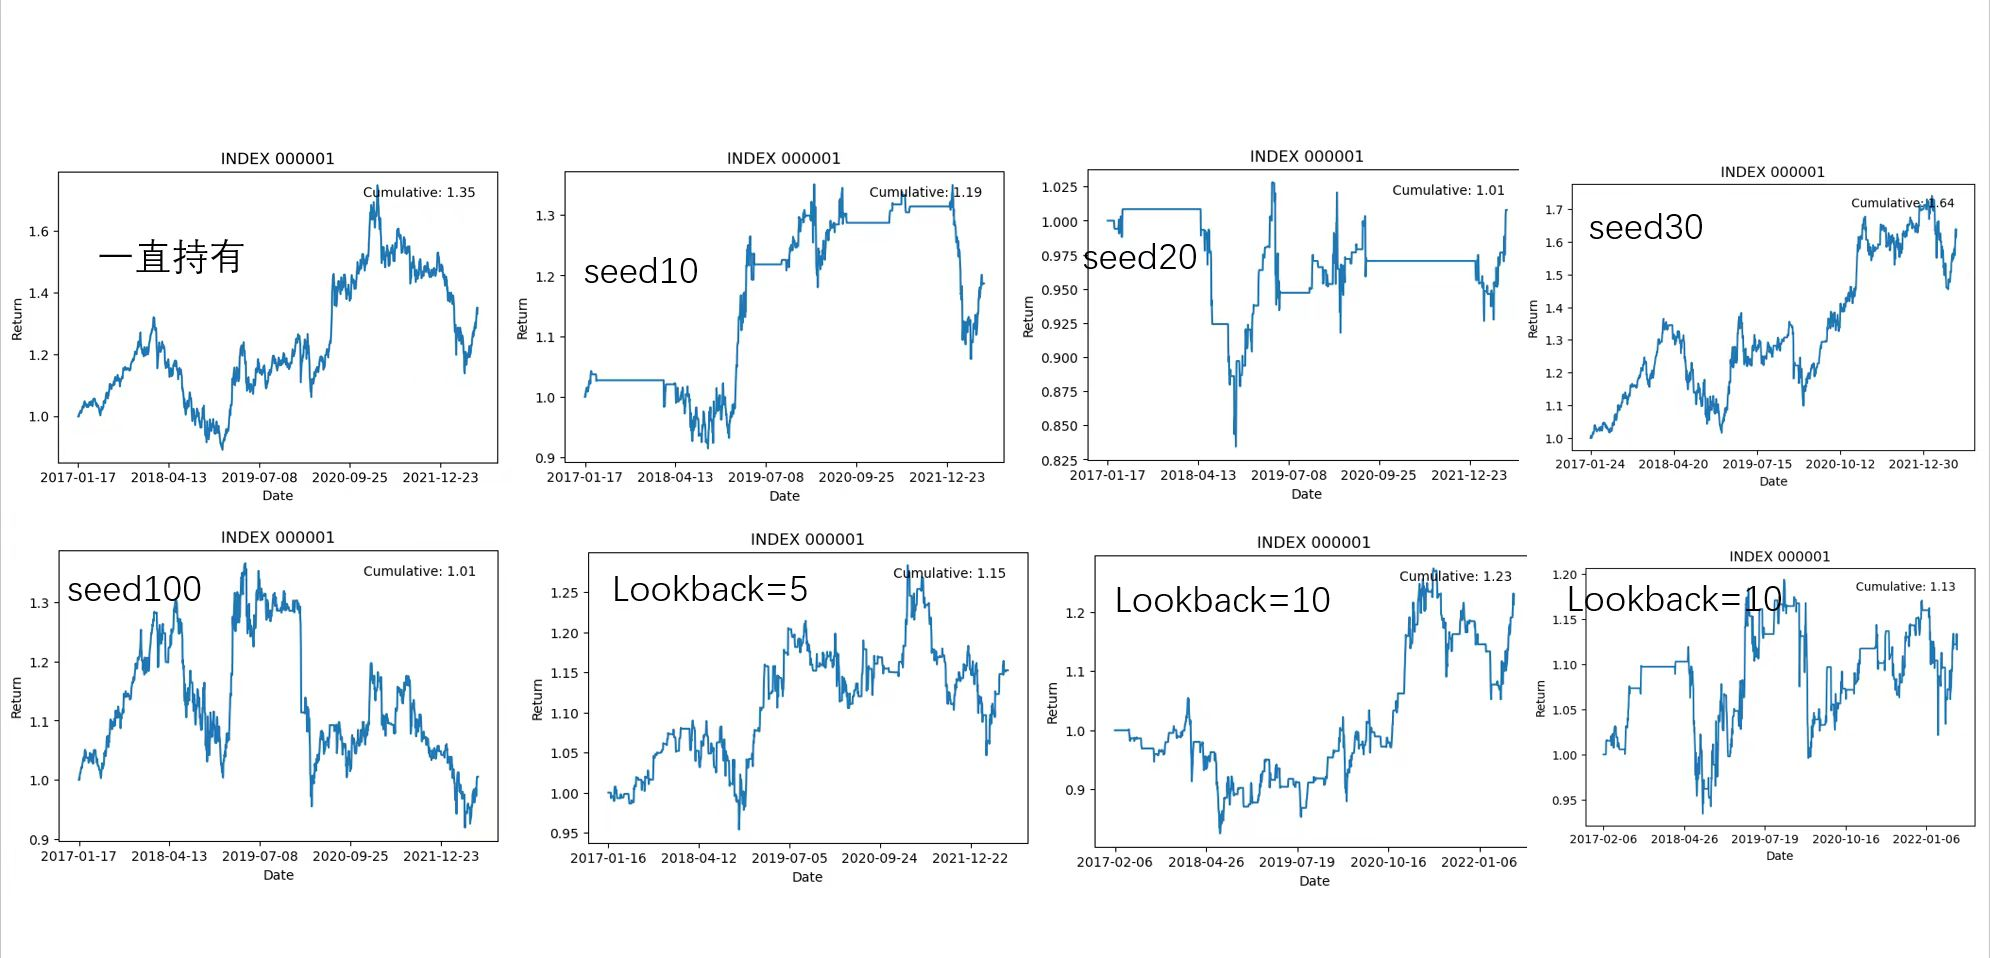
\includegraphics[width=10cm]{../fig/result.jpg}
\end{figure}


\end{frame}

\begin{frame}
\frametitle{谢谢!}
\begin{figure}
\centering
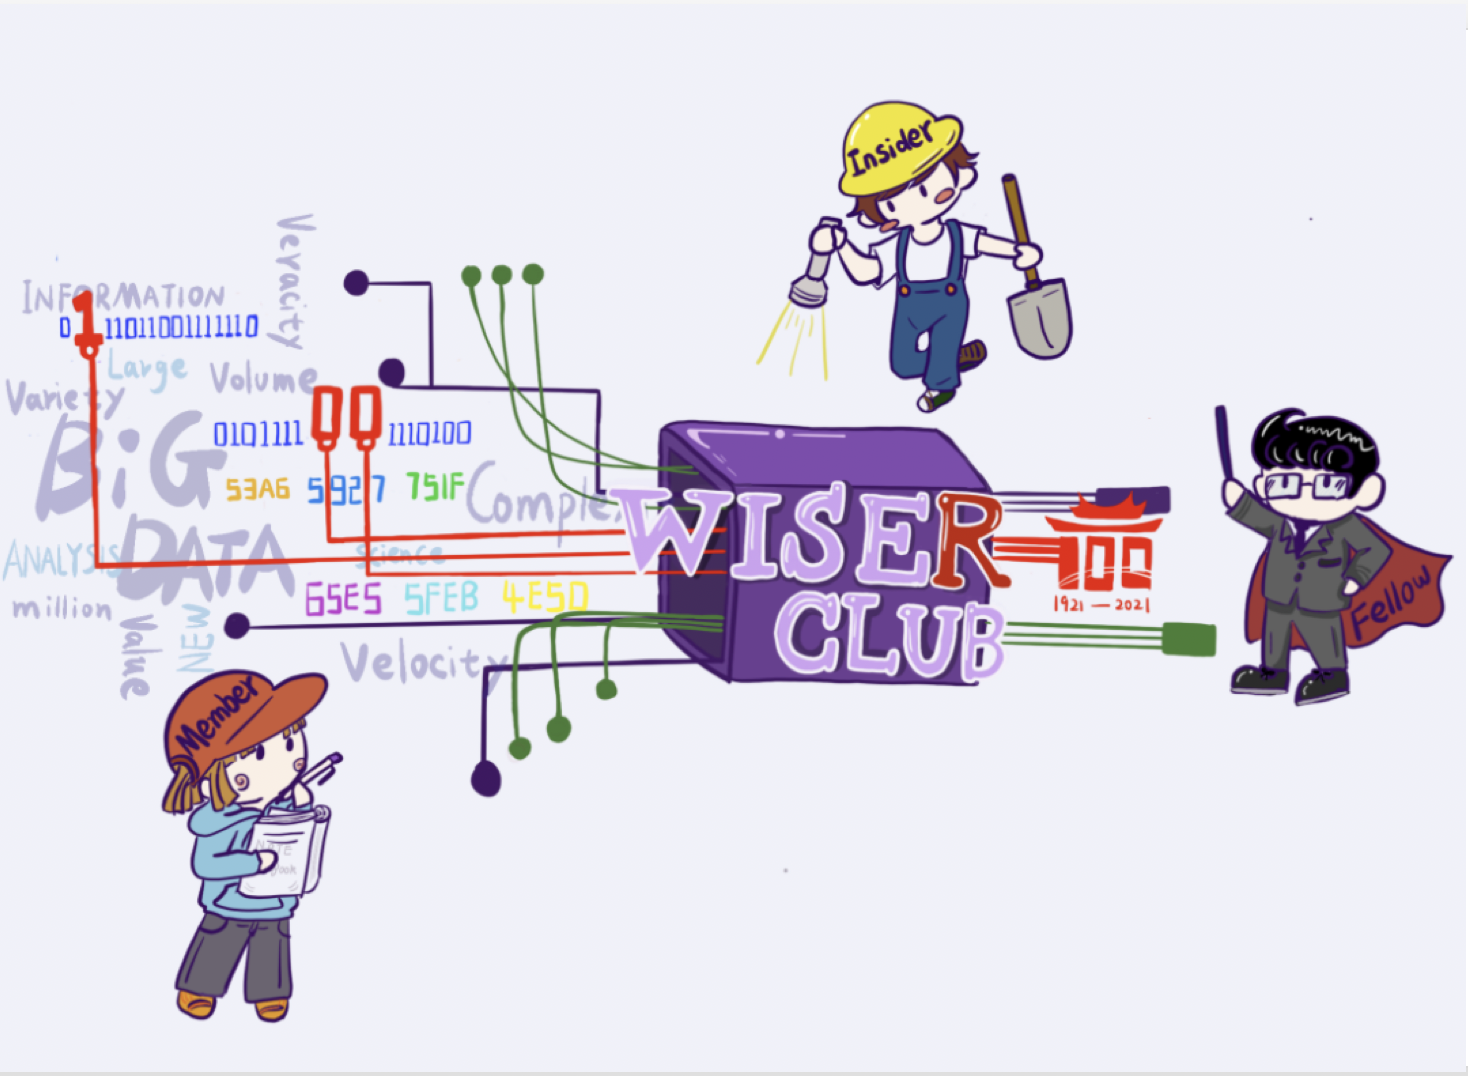
\includegraphics[width=10cm]{../fig/wiserclub.png}
\end{figure}
\end{frame}










\end{document} 